\chapter{Hints}

\begin{enumerate}[label=\textbf{H\arabic*.}]
    \item Factor $n^2 + n$.
    \item Use $p \mid P(a + kp_1) - P(a)$ to prove that $P(x)$ has infinitely many points $m_i$ such that $P(m_i) = p_1$.
    \item Use the fact that $\gcd(kx, ky) = k \cdot \gcd(x, y)$.
    \item Identify the critical points where each argument of the absolute value (what's inside the absolute value bars) changes from positive to negative ($=0$). Split into cases using these.
    \item Use the Polynomial Division Theorem (Theorem 3.3). 
    \item Let the finite set of primes $\equiv -1 \pmod{4}$ be 
    
    \noindent $\{p_1, p_2, \ldots, p_k\}$. Consider the integer
    \[
    N = 4p_1p_2\cdots p_k -1
    \]
    and analyze $\pmod{4}$.
    \item Use the last two facts to rewrite $(p-1)!$
    \[
    (p-1)! \equiv  \left( \frac{p-1}{2} \right)! \cdot  (-1)^{\frac{p-1}{2}}\left( \frac{p-1}{2} \right)! 
    \]
    \item Take the mod! Though this one is not as obvious.
    \item Use proof by contradiction.
    \item Do a proof by Contradiction, similar to Problem 4.1
    \item Don't assume it is true just because I told you so!
    \item As with the proof of the infinitude of primes, consider a proof by contradiction.
    \item Note that $\forall k, \forall a, a-k \equiv -k \pmod{a}$.
    \item Write $A'$ and $B'$ in terms of these 4 spaces. 
    \item Set some $P(a) = p_1$ to use the aforementioned theorem.
    \item Try to find a counterexample to 
    \[
    \gcd(a+b, ab) = \gcd(a, b)
    \]
    \item Can $a^5b$ or $ab^5 \equiv 6 \pmod{9}$?
    \item For the sum, pair element such that they add to $0$. Pair an element with its additive inverse.
    \item Consider the arcs subtended by the diagonals and turn the equality statement into a statement using arcs.
    \item Can you make a $0$ or $1 \pmod{9}$ using $7$ and $5$?
    \item Prove $AB$ is a diameter of the circumcircle by considering how it splits the circle into 2 arcs.
    \item  Consider the Binomial Theorem. 
    \[
    (a+b)^n = 
    \]
    \[
    \binom{n}{0}a^nb^0 + \binom{n}{1}a^{n-1}b^1 + \cdots + \binom{n}{n-1}a^1b^{n-1} + \binom{n}{n}a^0b^n
    \]
    \[
    = \sum_{i=0}^{n}\binom{n}{i}a^{n-i}b^i
    \]
    \item Prove for all primes $p > 3$ there exists no solution to the equation by taking the mod.
    \item $a^5b \cdot ab^5 = a^6b^6 = (ab)^6$ so consider 6th powers $\pmod{9}$.
    \item Find $A' \cup B'$ and $A' \cap B'$, in terms of these 4 spaces. Relate these to $(A \cup B)'$ and $(A \cap B)'$ visually or algebraically (again in terms of the 4 spaces). 
    \item Use a triangle/stairstep pattern. Row 1 has one dot, Row 2 has 2 dots, and so on. Try to see if you can explain it and get the formula $\frac{n(n+1)}{2}$ from here!
    \item Find $\sin(\angle ACD)$ (remember, $\sin$ is $\frac{opposite}{hypotenuse}$).
    \item The sum of all divisors of a number
    \[ 
    n = p_1^{e_1}p_2^{e_2} \cdots p_n^{e_n}
    \]
    \[
    = \prod_{i=1}^{n}{p_i^{e_i}}
    \]
    is
    \[
    s(n) = 
    \]
    \[
    (1 + p_1 + \cdots + p_1^{e_1})(1 + p_2 + \cdots + p_2^{e_2})\cdots(1 + p_n + \cdots + p_n^{e_n})
    \]
    \[
    = \prod_{i=1}^{n}{\left( \sum_{j = 0}^{e_i}{p_i^{j}} \right)}
    \]
    \item Use angle-angle similarity to prove similar triangles. 
    \item Just for book-keeping, note that $\angle A = \angle BAC$, $\angle B = \angle ABC$, $\angle C = \angle ACB$. The sides are such that side $a$ is opposite of angle $\angle A$, side $b$ is opposite of angle $\angle B$, and side $c$ is opposite of angle $\angle C$.
    \item Consider $P(a + kp_1) - P(a)$ for all $k$.
    \item $2^p = 3^q$. Find the contradiction, for integers $p$ and $q$. 
    \item Consider the formula for "n choose k"
    \[
    \binom{n}{k} = \frac{n!}{k!(n-k)!}
    \]
    and note the factors in the denominator vs numerator.
    \item Prove
    \[
    a^2 + b^2 + c^2 \geq ab + bc + ca
    \]
    by applying AM-GM to pairs of terms squared (i.e. $a^2$ and $b^2$). 
    \item The inverse of $-1$ in any mod is $-1$. Thus, the inverse of $(-1)^{\frac{p-1}{2}}$ is also $(-1)^{\frac{p-1}{2}}$. 
    \item Prove that chords are equal if and only if those chords subtend equal arcs using triangle congruence and considering the central angles.
    \item Sum the evaluations of each of the 2025 pairs to simplify the denominator.
    \item Use the polynomial division theorem (Theorem 3.3). 
    \item We can use symmetry. Prove that, for example, 
    \[
    \frac{b}{\sin B} = 2R
    \]
    and the proof for the others, $\frac{a}{\sin A}$ and $\frac{c}{\sin C}$, will follow the same up to symmetry.
    \item Split into two statements using the fact that if $x \equiv 0 \pmod{ab}$ and $\gcd(a, b) = 1$, then $x \equiv 0 \pmod{a}$ and $x \equiv 0 \pmod{b}$. 
    \item You know the drill! Consider a mod that is restrictive on perfect squares. (Or consider both and see which one works).
    \item Try a direct proof using the formula for the sum of the proper divisors of a number (not exactly the formula I gave you last hint). You may find it beneficial to use summation and/or product notation with $\sum$ and $\prod$, but if you find $\ldots$ easier to work with then use that instead.
    \item Set $\gcd(a, b) = k$ so $a = \alpha k$ and $b = \beta k$.
    \item Try $\pmod{4}$.
    \item Rewrite the expansion of $(r_1 + r_2 + r_3)^2$ in terms of what we can find using Vieta's formulas. Isolate the unknown quantity and map the other side of the equation to things we can find via Vieta's. 
    \item Derive a contradiction using the fact that a polynomial cannot have an infinite number of roots/infinite degree (by the definition of a polynomial). 
    \item Consider the residues $\pmod{4}$ to try to obtain the contradiction.
    \item Use $\pmod{3}$. Can $p^2 \equiv 0 \pmod{3}$?
    \item Consider reducing the expression by taking the mod of both sides with a small number, and use this to identify constraints on the left-hand side.
    \item Draw a figure. Then, let $O$ be the center of the circle. What is $\angle AOB$?
    \item For the $\pmod{q}$ case, write everything (including $(p-1)!$) in terms of $q = p+2$. You will find it easier to simplify using negative residues $\pmod{(p+2)}$. 
    \item Try reducing the expression by taking the modulo of both sides, and reasoning using the restrictions on perfect squares under mods (perfect squares sometimes cant be equal to certain residues under certain mods).
    \item Try $\pmod{9}$.
    \item $N \equiv 3 \pmod{4}$, and so its factors must be $1$ or $3 \pmod{4}$. 
    \item What is $a^5b$ and $ab^5 \pmod{9}$?
    \item Group the sum by pairs. Use Vieta's formulas to each quadratic factor $kx^2 - 4x - 3$ to evaluate each pair $\frac{1}{r_{2k-1}} + \frac{1}{r_{2k}}$. 
    \item Each element in the original set has $2$ choices: either it is in the subset or not. Think of each subset being represented by these sequences of "in/out" decisions. 
    \item Use the vertical angle theorem. This is a pretty intuitive idea, but still worth noting explicitly. Given straight lines $AB$ and $CD$ which intersect and point $E$,
    \begin{center}
    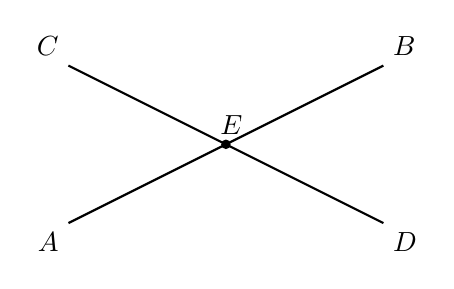
\begin{tikzpicture}
    % Draw two intersecting lines
    \draw[thick] (-2,-1) -- (2,1);
    \draw[thick] (-2,1) -- (2,-1);
    
    % Label the points for Line 1 (AB) and Line 2 (CD)
    \node at (-2,-1) [below left] {$A$};
    \node at (2,1) [above right] {$B$};
    \node at (-2,1) [above left] {$C$};
    \node at (2,-1) [below right] {$D$};
    
    % Intersection point E with a small dot
    \filldraw (0,0) circle (1.5pt) node[above, xshift=2pt] {$E$};
    \end{tikzpicture}
    \end{center}
    $\angle AEC = \angle DEB$ and $\angle CEB = \angle DEA$. 
    \item Use the identity 
    \[
    1 + 2 + 4 + \cdots 2^{k-1} = 2^k-1
    \]
    \item The easiest method of proof here is probably proof by contrapositive.
    \item Use a property of cyclic quadrilaterals to relate $\angle B$ and $\angle ACD$.
    \item Use casework on the parity of $n$ since $(-1)^n$ behaves differently for odd and even $n$.
    \item Only need one similarity (either works) to prove the Power of a Point result. Use the common ratio between sides in similar triangles. 
    \item For two sets $A$ and $B$, $|A| = |B|$ if there is a one-to-one map between elements of both sets such that every element of $A$ maps to a unique element of $B$ and every element of $B$ maps backwards to a unique element of $A$. This is known as a bijection.
    \item "Undo" the $\log$ to get 
    \[something ~ with ~ 2 = something~ with ~ 3\]
    \item Reduce via $\pmod{4}$ so we don't have to worry about the $4m$ term. 
    \item Since $N \equiv 3 \pmod{4}$, it must have at-least one factor $\equiv 3 \pmod{4}$. 
    \item $(p+1)! = (p-1)! (p)(p+1) $. 
    \[
    (p+1)! \equiv (p-1)! (-2)(-1) \pmod{(p+2)}
    \]
    \item Prove using contradiction (or another method if you feel it may be appropriate) that
    \[
    \gcd(\alpha, \beta) = 1 \implies \gcd(\alpha + \beta, \alpha\beta) = 1
    \]
    and apply this lemma appropriately.
    \item Check small primes and see if there are solutions. 
    \item Think of it as a shopping list to construct subsets! For every element in the original set, to construct a subset, we can choose to either add the element to our subset or leave it. 
    \item Expand $(r_1 + r_2 + r_3)^2$.
    \item Use the fact that $ab \mid x \implies a \mid x \text{ and } b \mid x$.
    \item The case of $\equiv 0 \pmod{p}$ is easy if you use Wilson's Theorem.
    \item This is a trick question!
    \item Consider $\pmod{3}$ and $\pmod{4}$. First compute manually (there's not a better way) of the resides that perfect squares can attain in these mods.
    \item Split into cases by parity of $a$ and $b$ which satisfy the premise of the contrapositive (the "if" part). 
    \item Break up the entire universe $U$ into 4 spaces. Only $A$, only $B$, $A \cap B$, and the rest of the universe. Draw these in a Venn diagram.
    \item Consider Euclid's Lemma, which states that for any prime number $p$
    \[
    p \mid ab \iff (p \mid a \text{ or } p \mid b)
    \]
    \item Prove that 
    \[
    \gcd(x, y) = 1 \implies \gcd(x, yz) = \gcd(x, z)
    \]
    and use this lemma appropriately. 
    \item For now, sets can contain themselves. We defined a set to be a collection of things, and so there's nothing wrong with this! (for now)
    \item Prove via algebraic manipulation (direct proof) that
    \[
    ab + bc + ca = \frac{1-(a^2+b^2+c^2)}{2}
    \]
    \item A proper divisor is a divisor of a number that is not itself. I.e. the proper divisors of $6$ are $\{1, 2, 3\}$ while the full set of divisors of $6$ is $\{1, 2, 3, 6\}$.
    \item Use the fact that inscribed angles that subtend the same arc are equal. 
    \item Simplify $\frac{1}{r_{2k-1}} + \frac{1}{r_{2k}}$ by combining over a common denominator.
    \item 6th powers can only be $\equiv 0, 1 \pmod{9}$.
    \item Rearrange the $(p-1)!$ into 
    \[
    (p-1)! = 1 \cdot 2 \cdots \left(\frac{p-1}{2}\right) \cdot \left(  p-\frac{p-1}{2} \right) \cdots (p-2) \cdot (p-1)
    \]
    \item Assuming you are proving $\frac{b}{\sin B} = 2R$, draw in point $D$ such that $AD$ is a diameter, and find $\angle ACD$. 
\end{enumerate}




\begin{comment}
Chapter 1. 

1.4
H1: Use a triangle/stairstep pattern. Row 1 has one dot, Row 2 has 2 dots, and so on. Try to see if you can explain it and get the formula $\frac{n(n+1)}{2}$ from here!



Chapter 2

2.2
H2: Break up the entire universe $U$ into 4 spaces. Only $A$, only $B$, $A \cap B$, and the rest of the universe. Draw these in a Venn diagram.
H3: Write $A'$ and $B'$ in terms of these 4 spaces. 
H4: Find $A' \cup B'$ and $A' \cap B'$, in terms of these 4 spaces. Relate these to $(A \cup B)'$ and $(A \cap B)'$ visually or algebraically (again in terms of the 4 spaces). 

2.3
H5: For two sets $A$ and $B$, $|A| = |B|$ if there is a one-to-one map between elements of both sets such that every element of $A$ maps to a unique element of $B$ and every element of $B$ maps backwards to a unique element of $A$. This is known as a bijection.

2.6
H6: Think of it as a shopping list to construct subsets! For every element in the original set, to construct a subset, we can choose to either add the element to our subset or leave it. 
H7: Each element in the original set has $2$ choices: either it is in the subset or not. Think of each subset being represented by these sequences of "in/out" decisions. 

2.7
H8: For now, sets can contain themselves. We defined a set to be a collection of things, and so there's nothing wrong with this! (for now)



Chapter 3

3.1
H9: Factor $n^2 + n$.

3.3
H10: Identify the critical points where each argument of the absolute value (what's inside the absolute value bars) changes from positive to negative ($=0$). Split into cases using these. 

3.4
H11: Consider Euclid's Lemma, which states that for any prime number $p$
\[
p \mid ab \iff (p \mid a \text{ or } p \mid b)
\]

3.8
H12: Prove via algebraic manipulation (direct proof) that
\[
ab + bc + ca = \frac{1-(a^2+b^2+c^2)}{2}
\]
H13: Prove
\[
a^2 + b^2 + c^2 \geq ab + bc + ca
\]
by applying AM-GM to pairs of terms squared (i.e. $a^2$ and $b^2$). 

3.9
H14: Use the Polynomial Division Theorem (Theorem 3.3). 

3.10
H15: Expand $(r_1 + r_2 + r_3)^2$
H16: Rewrite the expansion of $(r_1 + r_2 + r_3)^2$ in terms of what we can find using Vieta's formulas. Isolate the unknown quantity and map the other side of the equation to things we can find via Vieta's. 

3.11
H17: Simplify $\frac{1}{r_{2k-1}} + \frac{1}{r_{2k}}$ by combining 
over a common denominator.
H18: Group the sum by pairs. Use Vieta's formulas to each quadratic factor $kx^2 - 4x - 3$ to evaluate each pair $\frac{1}{r_{2k-1}} + \frac{1}{r_{2k}}$. 
H19: Sum the evaluations of each of the 2025 pairs to simplify the denominator.

3.12
H20: Try reducing the expression by taking the modulo of both sides, and reasoning using the restrictions on perfect squares under mods (perfect squares sometimes cant be equal to certain residues under certain mods).
H21: Consider $\pmod{3}$ and $\pmod{4}$. First compute manually (there's not a better way) of the resides that perfect squares can attain in these mods.
H22: Use casework on the parity of $n$ since $(-1)^n$ behaves differently for odd and even $n$.



Chapter 4

4.2
H23: Consider reducing the expression by taking the mod of both sides with a small number, and use this to identify constraints on the left-hand side.
H24: Reduce via $\pmod{4}$ so we don't have to worry about the $4m$ term. 

4.3
H25: The easiest method of proof here is probably proof by contrapositive.
H26: Split into cases by parity of $a$ and $b$ which satisfy the premise of the contrapositive (the "if" part). 

4.5
H27: Do a proof by Contradiction, similar to Problem 4.1
H28: "Undo" the $\log$ to get $something ~ with ~ 2 = something~ with ~ 3$
H29: $2^p = 3^q$. Find the contradiction, for integers $p$ and $q$. 

4.6
H30: You know the drill! Consider a mod that is restrictive on perfect squares. (Or consider both and see which one works)
H31: Try $\pmod{4}$.

4.7
H32: Draw a figure. Then, let $O$ be the center of the circle. What is $\angle AOB$?
H33: Prove $AB$ is a diameter of the circumcircle by considering how it splits the circle into 2 arcs.

4.8
H34: As with the proof of the infinitude of primes, consider a proof by contradiction.
H35: Consider the residues $\pmod{4}$ to try to obtain the contradiction.
H36: Let the finite set of primes $\equiv -1 \pmod{4}$ be $\{p_1, p_2, \ldots, p_k\}$. Consider the integer
\[
N = 4p_1p_2\cdots p_k -1
\]
and analyze $\pmod{4}$.
H37: $N \equiv 3 \pmod{4}$, and so its factors must be $1$ or $3 \pmod{4}$. 
H38: Since $N \equiv 3 \pmod{4}$, it must have at-least one factor $\equiv 3 \pmod{4}$. 

4.9
H39: Take the mod! Though this one is not as obvious.
H40: Try $\pmod{9}$.
H41: What is $a^5b$ and $ab^5 \pmod{9}$?
H42: Can $a^5b$ or $ab^5 \equiv 6 \pmod{9}$?
H43: $a^5b \cdot ab^5 = a^6b^6 = (ab)^6$ so consider 6th powers $\pmod{9}$.
H44: 6th powers can only be $\equiv 0, 1 \pmod{9}$.
H45: Can you make a $0$ or $1 \pmod{9}$ using $7$ and $5$?



Chapter 5

5.1
H46: Try to find a counterexample to $\gcd(a+b, ab) = \gcd(a, b)$.
H47: Set $\gcd(a, b) = k$ so $a = \alpha k$ and $b = \beta k$. 
H48: Use the fact that $\gcd(kx, ky) = k \cdot \gcd(x, y)$.
H49: Prove using contradiction (or another method if you feel it may be appropriate) that
\[
\gcd(\alpha, \beta) = 1 \implies \gcd(\alpha + \beta, \alpha\beta) = 1
\]
and apply this lemma appropriately.
H50: Prove that 
\[
\gcd(x, y) = 1 \implies \gcd(x, yz) = \gcd(x, z)
\]
and use this lemma appropriately. 

5.2
H51: Prove that chords are equal if and only if those chords subtend equal arcs using triangle congruence and considering the central angles.
H52: Consider the arcs subtended by the diagonals and turn the equality statement into a statement using arcs.

5.3
H53: For the sum, pair element such that they add to $0$. Pair an element with its additive inverse.

5.4
H54: Use the fact that inscribed angles that subtend the same arc are equal. 
H55: Use the vertical angle theorem. This is a pretty intuitive idea, but still worth noting explicitly. Given straight lines $AB$ and $CD$ which intersect and point $E$,
\begin{center}
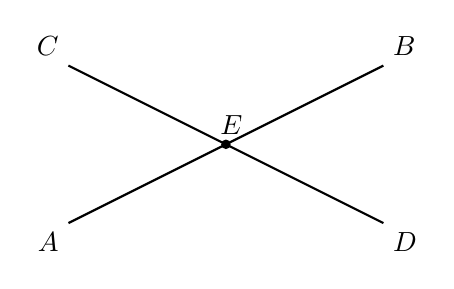
\begin{tikzpicture}
    % Draw two intersecting lines
    \draw[thick] (-2,-1) -- (2,1);
    \draw[thick] (-2,1) -- (2,-1);
    
    % Label the points for Line 1 (AB) and Line 2 (CD)
    \node at (-2,-1) [below left] {$A$};
    \node at (2,1) [above right] {$B$};
    \node at (-2,1) [above left] {$C$};
    \node at (2,-1) [below right] {$D$};
    
    % Intersection point E with a small dot
    \filldraw (0,0) circle (1.5pt) node[above, xshift=2pt] {$E$};
\end{tikzpicture}
\end{center}
$\angle AEC = \angle DEB$ and $\angle CEB = \angle DEA$. 
H56: Use angle-angle similarity to prove similar triangles. 
H57: Only need one similarity (either works) to prove the Power of a Point result. Use the common ratio between sides in similar triangles. 

5.5
H58: Rearrange the $(p-1)!$ into 
\[
(p-1)! = 1 \cdot 2 \cdots \left(\frac{p-1}{2}\right) \cdot \left(  p-\frac{p-1}{2} \right) \cdots (p-2) \cdot (p-1)
\]
H59: Note that $\forall k, \forall a, a-k \equiv -k \pmod{a}$.
H60: Use the last two facts to rewrite $(p-1)!$
\[
(p-1)! \equiv  \left( \frac{p-1}{2} \right)! \cdot  (-1)^{\frac{p-1}{2}}\left( \frac{p-1}{2} \right)! 
\]
H61: The inverse of $-1$ in any mod is $-1$. Thus, the inverse of $(-1)^{\frac{p-1}{2}}$ is also $(-1)^{\frac{p-1}{2}}$. 

5.6
H62: Use proof by contradiction.
H63: Use the polynomial division theorem (Theorem 3.3). 
H64: Set some $P(a) = p_1$ to use the aforementioned theorem.
H65: Consider $P(a + kp_1) - P(a)$ for all $k$.
H66: Use the fact that $ab \mid x \implies a \mid x \text{ and } b \mid x$.
H67: Derive a contradiction using the fact that a polynomial cannot have an infinite number of roots/infinite degree (by the definition of a polynomial). 
H68: Use $p \mid P(a + kp_1) - P(a)$ to prove that $P(x)$ has infinitely many points $m_i$ such that $P(m_i) = p_1$.

5.7
H69: This is a trick question!
H70: Don't assume it is true just because I told you so!

5.8
H71: Split into two statements using the fact that if $x \equiv 0 \pmod{ab}$ and $\gcd(a, b) = 1$, then $x \equiv 0 \pmod{a}$ and $x \equiv 0 \pmod{b}$. 
H72: The case of $\equiv 0 \pmod{p}$ is easy if you use Wilson's Theorem.
H73: For the $\pmod{q}$ case, write everything (including $(p-1)!$) in terms of $q = p+2$. You will find it easier to simplify using negative residues $\pmod{(p+2)}$. 
H74: $(p+1)! = (p-1)! (p)(p+1) $. 
\[
(p+1)! \equiv (p-1)! (-2)(-1) \pmod{(p+2)}
\]

5.9
H75: A proper divisor is a divisor of a number that is not itself. I.e. the proper divisors of $6$ are $\{1, 2, 3\}$ while the full set of divisors of $6$ is $\{1, 2, 3, 6\}$.
H76: The sum of all divisors of a number
\[ 
n = p_1^{e_1}p_2^{e_2} \cdots p_n^{e_n} = \prod_{i=1}^{n}{p_i^{e_i}}
\]
is
\[
s(n) = (1 + p_1 + \cdots + p_1^{e_1})(1 + p_2 + \cdots + p_2^{e_2})\cdots(1 + p_n + \cdots + p_n^{e_n})
\]
\[
= \prod_{i=1}^{n}{\left( \sum_{j = 0}^{e_i}{p_i^{j}} \right)}
\]
H77: Try a direct proof using the formula for the sum of the proper divisors of a number (not exactly the formula I gave you last hint). You may find it beneficial to use summation and/or product notation with $\sum$ and $\prod$, but if you find $\ldots$ easier to work with then use that instead.
H78: Use the identity $1 + 2 + 4 + \cdots 2^{k-1} = 2^k-1$.

5.10
H79: Consider the formula for "n choose k"
\[
\binom{n}{k} = \frac{n!}{k!(n-k)!}
\]
and note the factors in the denominator vs numerator.
H80: Consider the Binomial Theorem. 
\[
(a+b)^n = \binom{n}{0}a^nb^0 + \binom{n}{1}a^{n-1}b^1 + \cdots + \binom{n}{n-1}a^1b^{n-1} + \binom{n}{n}a^0b^n
\]
\[
= \sum_{i=0}^{n}\binom{n}{i}a^{n-i}b^i
\]

5.11
H81: Check small primes and see if there are solutions. 
H82: Prove for all primes $p > 3$ there exists no solution to the equation by taking the mod.
H83: Use $\pmod{3}$. Can $p^2 \equiv 0 \pmod{3}$?

5.12
H84: Just for book-keeping, note that $\angle A = \angle BAC$, $\angle B = \angle ABC$, $\angle C = \angle ACB$. The sides are such that side $a$ is opposite of angle $\angle A$, side $b$ is opposite of angle $\angle B$, and side $c$ is opposite of angle $\angle C$.
H85: We can use symmetry. Prove that, for example, 
\[
\frac{b}{\sin B} = 2R
\]
and the proof for the others, $\frac{a}{\sin A}$ and $\frac{c}{\sin C}$, will follow the same up to symmetry.
H86: Assuming you are proving $\frac{b}{\sin B} = 2R$, draw in point $D$ such that $AD$ is a diameter, and find $\angle ACD$. 
H87: Use a property of cyclic quadrilaterals to relate $\angle B$ and $\angle ACD$.
H88: Find $\sin(\angle ACD)$ (remember, $\sin$ is $\frac{opposite}{hypotenuse}$).
\end{comment}